\documentclass[pdflatex,sn-mathphys-num]{sn-jnl}
\usepackage{textcomp,xcolor,amsmath,amssymb,graphicx,booktabs,tabularx,longtable,adjustbox,placeins,xurl}
\usepackage{journal-reading-layout}
\hypersetup{hidelinks}
\let\burl\url
\setlength{\emergencystretch}{2em}
\newcommand{\ind}{\mathbf{1}}
\raggedbottom
\errorcontextlines=100
\begin{document}
\title{Evaluating Deadline-Limited Communication in Multi-Agent Reinforcement Learning: Delivery, Computation, and Control}
\author[1]{\fnm{Yeong-woo} \sur{Kung}}\email{yeongwoo@konkuk.ac.kr}
\author*[1]{\fnm{Young-guk} \sur{Ha}}\email{ygha@konkuk.ac.kr}
\affil[1]{\orgdiv{Smart Computing Laboratory, Department of Computer Science \& Engineering}, \orgname{Konkuk University}, \orgaddress{\street{120 Neungdong-ro, Gwangjin-gu}, \city{Seoul}, \postcode{05029}, \country{Republic of Korea}}}
\abstract{Communication-efficient multi-agent reinforcement learning is often assessed through communication cost and task performance. Prior work also studies sender scheduling, buffered messages, delay-aware reception and behavioral responses to messages. These distinct concerns motivate a narrower question: which mechanisms can a cost--performance comparison identify when communication and action computation face deadlines? We analyze this question through matched-policy interventions in Oracle-assisted Hallway, Oracle-free hidden-source broadcast and a reconstruction of the MNIST-sum game. Our analysis separates offered traffic from received information, sender sensitivity from selection advantage, and decodable information from executed control. In Hallway, an 80\% reduction in offered traffic preserves every received update, action and reward across 400 paired episodes. Equal received counts outside this boundary conceal different sender histories. Feasible sender substitutions change some outcomes, but do not establish a consistent episode-weighted advantage for the evaluated priority rule. In broadcast, supervised receiver adaptation retains a 5.63-percentage-point gain when late actions are replaced by the previous executed action. The favorable results have explicit boundaries: readiness uncertainty and decision overhead can reverse an admission advantage, and sufficiently late computation eliminates the receiver gain. These findings support a four-stage protocol for validating learned communication, tracing delivery and cost, isolating sender choice, and testing receiver use. They concern the evaluated policies and timing models, rather than failures of the cited native methods or generalization to standard sequential benchmarks.}
\keywords{Multi-agent reinforcement learning, Communication scheduling, Deadline constraints, Message selection, Controlled evaluation}
% Names-only reading front matter; complete submission metadata is in title_page.tex.
\pagestyle{headings}
\begingroup
\makeatletter
{\Titlefont\@title\par}
\makeatother
\vspace{10pt}
{\Authorfont Yeong-woo Kung \enspace\textperiodcentered\enspace Young-guk Ha\par}
\vspace{12pt}
\printabstract
\printkeywords
\endgroup
\vspace{10pt}
\section{Introduction}
Communication-efficient multi-agent reinforcement learning (MARL) aims to preserve cooperative performance while reducing information exchange. Variance-based control (VBC) reports return and communicating-pair overhead~\citep{zhang2019efficient}; temporal message control (TMC) evaluates reduced exchanges and tolerance to transmission loss~\citep{zhang2020succinct}; SchedNet compares learned scheduling with round-robin and full communication~\citep{kim2019schedule}. These studies motivate communication reduction and selective access. Our question concerns the interpretation of such outcomes when packets and actions must meet deadlines: what has actually changed between the communication decision and the executed action?

Three ambiguities motivate our analysis. A suppressed packet may already have been too late to arrive, so a traffic saving need not remove receiver information. Equal received counts may hide different senders and retained histories, so a performance difference need not identify present sender-selection quality. Finally, information may be available in a receiver input without improving the action that is actually executed. Behavioral listening~\citep{lowe2019pitfalls} and delay-aware waiting~\citep{yuan2023dacom} make the latter questions explicit, but answering them together requires controls over reception, policy state and computation.

We study these ambiguities using existing learned policies in Oracle-assisted five-agent Hallway, Oracle-free hidden-source broadcast and a reconstruction of the MNIST-sum game. The cited literature supplies the analysis targets; our own paired interventions supply the findings. This is a focused experimental analysis of attribution under deadlines, not a systematic review or a re-evaluation of every cited method in its native benchmark. Four stages organize the analysis: validate the learned reference, account for delivery and computation, isolate sender choice, and test downstream information use. The contributions are:
\begin{enumerate}
\item A delivery-level explanation of traffic savings. In Hallway, 80\% fewer offered bytes preserve every delivered update, action and reward across 400 paired episodes. Beyond this boundary, equal received counts conceal different histories.
\item Controlled tests of sender choice and memory. Feasible substitutions change suffix return in 13.9--18.9\% of sampled states, but all four episode-weighted factual-minus-uniform intervals include zero. Shared histories and cache removal reveal why behavioral effects and reward effects must be reported separately.
\item Tests of useful reception and executed control. Timing-informed admission improves MNIST-sum accuracy at equal offered cost under known readiness. Supervised receiver adaptation retains a 5.63-point broadcast gain with previous-action fallback, while readiness uncertainty and additional computation delimit these benefits.
\end{enumerate}
The contribution is the evidence connecting each interpretation to its control. We retain the no-message Hallway solution and failed learning/replay gates because they restrict what these experiments establish. Section~\ref{sec:related} identifies the literature basis; Sections~\ref{sec:problem} and~\ref{sec:design} define the controls and tasks. Section~\ref{sec:results} reports the findings, followed by their implications and limits in Section~\ref{sec:discussion}.

\section{Related work and analysis targets}\label{sec:related}
\subsection{Why analyze delivery, selection and history?}
Communication surveys organize design choices such as whom, what and when to communicate~\citep{zhu2024survey}. Learned channels, aggregation and targeted communication provide ways to condition actions on remote information~\citep{foerster2016learning,sukhbaatar2016learning,das2019tarmac}; triggering and information bottlenecks further constrain exchange~\citep{hu2023event,wang2020imac}. We select evaluation mechanisms represented by these designs, rather than rank the methods. Each target below has an identifiable source practice, a possible ambiguity under our deadline model, and a corresponding intervention.

\textbf{Traffic and delivery.} VBC, Section~6.2, measures the fraction of communicating agent pairs alongside its performance evaluation~\citep{zhang2019efficient}. TMC, Sections~5.2--5.3, separately evaluates communication overhead and transmission loss~\citep{zhang2020succinct}. These are useful system measurements. Under a reception cutoff, however, an attempted exchange and an available input are different events. We therefore compare offered wire bytes with sender-keyed payload traces, and use equal-cost admission to test whether matching traffic also matches useful reception (Sections~\ref{sec:identity}--\ref{sec:eccles}). This extension is our analytical question, not a claim that those papers established deadline-level equivalence.

\textbf{Sender choice and inherited information.} SchedNet jointly learns scheduling, encoding and acting; its Section~4 compares access schemes and describes a restricted-bandwidth DIAL baseline that retains messages from unscheduled agents~\citep{kim2019schedule}. TMC's Sections~4.1 and~4.3 explicitly maintain received-message buffers~\citep{zhang2020succinct}. These designs make both the current sender and previous receptions relevant. We ask whether a feasible replacement changes return, whether the factual selection exceeds uniform alternatives, and whether a contrast survives a shared starting history. Frozen weights, same-count substitutions and common-prefix branches address these separate questions (Sections~\ref{sec:selection}--\ref{sec:history}). Our DAC heuristic is not a reproduction of SchedNet.

\subsection{Why analyze readiness and receiver use?}
\textbf{Readiness and execution.} DACOM's architecture learns message-waiting thresholds through TimeNet~\citep{yuan2023dacom}. Update-age and task-oriented scheduling research likewise treats timing and control relevance as meaningful~\citep{kaul2012real,ayan2022semantics}. Our extension asks whether selector preparation and later action computation consume the opportunity being compared. Measured versus fixed readiness and rejection of late candidate actions test this on our implementation. They do not assess DACOM's native performance.

\textbf{Information and behavior.} Lowe et al., Sections~3.1--3.3, distinguish messages related to observations or actions from messages that influence a listener's behavior~\citep{lowe2019pitfalls}. Eccles et al., Sections~3--4, study signaling/listening biases and evaluate the MNIST-sum game~\citep{eccles2019biases}; Peters et al. review the interpretation of emergent-language metrics~\citep{peters2025emergent}. These sources motivate message interventions and a separation between available information and policy use. We reconstruct MNIST-sum to isolate one-step delivery, then use broadcast probes, true-label and shuffled-label head fitting, and fresh closed-loop rollouts to test behavioral gains. Our final extension asks whether those gains remain when late actions are rejected (Sections~\ref{sec:receiver_decision}--\ref{sec:deployment_robustness}).

\section{Evaluation framework}\label{sec:problem}
\subsection{Targets and paired interventions}
We record attempted wire bytes, timely sender-keyed payloads and timestamps, receiver state, CPU computation, executed actions and undiscounted return. For intervention $u$ and reference $v$, $n$ trained seeds and $E_s$ paired resets per seed, the episode-weighted contrast is
\begin{equation}
 \widehat{\Delta}_{u,v}=\frac{1}{n}\sum_{s=1}^{n}\frac{1}{E_s}
       \sum_{e=1}^{E_s}\bigl(G_{s,e}^{u}-G_{s,e}^{v}\bigr).
 \label{eq:episode_effect}
\end{equation}
A pair begins at matched resets or a copied full state; its later histories may diverge. Admission and sender interventions retain policy weights. Receiver adaptation deliberately changes the follower head while retaining other parameters. Independently trained access-rule comparisons are reported separately because their differences also include learning.

Table~\ref{tab:evaluation_protocol} connects each attribution question to its control. The stages are not an additive decomposition of return. A reference must first demonstrate learned communication use; reception traces then determine whether a traffic change reaches the policy at all. When received information differs, same-count substitutions test sender choice, whereas common-history branches and cache resets distinguish inherited state from current selection. Finally, held-out probes diagnose available information and fresh acting-head rollouts test whether it can improve behavior. Readiness and action-deadline accounting accompany these comparisons.
\begin{table}[htbp]\centering\normalsize
\caption{Questions and controls organizing the completed analysis. Each stage distinguishes a specific interpretation of a communication result; the tasks and interventions supporting it are identified in Section~\ref{sec:design}.}\label{tab:evaluation_protocol}
\begin{tabularx}{\textwidth}{@{}p{0.16\textwidth}XX@{}}
\toprule
Stage & Question & Control used in this study\\\midrule
Validate learning & Does the learned reference benefit from communication? & Learning checks, no-message comparisons and held-out message interventions; separate task-level controls.\\[3pt]
Account for delivery and cost & Does changing offered traffic change what arrives, and at what computation cost? & Matched-policy reception traces, equal-cost admission and measured versus fixed readiness.\\[3pt]
Isolate sender choice & Does sender identity matter, does the factual rule exploit it, and does the starting history change the comparison? & Same-count feasible substitutions, factual versus uniform choice, common-prefix branches and separate cache removal.\\[3pt]
Test receiver use & Can information in the received input improve the actions actually used? & Held-out probes, original/true-label/shuffled-label acting heads, fresh rollouts and rejection of late candidates.\\
\bottomrule\end{tabularx}
\end{table}

\subsection{Policies, reception and cost}
Hallway and broadcast use a shared GRU~\citep{cho2014learning} trained with QMIX~\citep{rashid2018qmix}. Local input contains observation, previous action and agent identity. A linear head produces eight float32 message entries; payload is $P=32$ B and modeled header is 16 B, giving wire size $S=48$ B. Received messages condition the action head rather than the recurrent update. Adam~\citep{kingma2015adam}, Double-Q targets~\citep{hasselt2016deepdouble}, discount 0.99 and the training settings are detailed in Supplementary Section~S1.

CPU inference uses one PyTorch thread and \texttt{perf\_counter\_ns}. Computation $C_t$ includes encoding, selection, byte serialization, cache operations, transport arithmetic, aggregation, action output and residual bookkeeping; environment stepping and logging are excluded. With packet readiness $P_{\mathrm{ready},t}$ and a fixed post-reception reserve $R_{\rm post}=0.45$ ms, the cutoff is $D_{\rm recv}=D_{\max}-R_{\rm post}$. Attempted senders are queued by $(i-t)\bmod N$, independently of priority score. For $K_t$ attempted packets, bandwidth $B$ and latency $\ell=0.05$ ms,
\begingroup\interdisplaylinepenalty=10000
\begin{align}
 A_{k,t}&=P_{\mathrm{ready},t}+kS/B+\ell,\nonumber\\ d_{k,t}&=\ind[A_{k,t}\le D_{\rm recv}],\\
 W_t&=\begin{cases}\min\!\left\{\begin{aligned}&K_tS/B+\ell,\\&[D_{\rm recv}-P_{\mathrm{ready},t}]_+\end{aligned}\right\},&K_t>0,\\0,&K_t=0,\end{cases}\\
 T_{\rm step,t}&=C_t+W_t.\label{eq:step}
\end{align}
\endgroup
Every attempted packet is charged in full, including cutoff drops. Accepted broadcasts reach all other agents; each step flushes the queue. Computation is measured and waiting is modeled, with no overlap, loss, collision, retry, acknowledgment or inter-step backlog. A miss occurs when $T_{\rm step,t}>D_{\max}$; the reception reserve does not replace measurement of later computation.

A timely message replaces its sender's cache payload and timestamp; otherwise both persist. Caches start zero and invalid. The receiver aggregate decays valid entries by age, excludes self-messages and divides by the number of valid senders. The action head also receives valid-neighbor count and mean age. Thus a delivery changes content, scaling and metadata. Supplementary Section~S8 gives the exact aggregate and accounting equations. Offered bytes, delivered payload, cache state, computation, deadline misses and return are distinct outcomes.

Full offers all senders; Periodic alternates them. Capacity-capped round-robin (RR) advances its cursor by the admitted count. DAC uses the same byte-credit and link caps but ranks local action-value gaps plus transmitter age. It is an evaluated heuristic. Physical score-collection traffic is not charged, although selector CPU work is measured. Matched-history tests hold cache decay fixed; Supplementary Section~S1 specifies cap, tie-breaking and reset rules.

\section{Experimental design}\label{sec:design}
\subsection{Tasks and learned references}
The three tasks answer different questions. Five-agent Hallway uses the CASEC/MACO implementation~\citep{wang2022casec}, including its preserved transition semantics. Groups of two and three agents must arrive together within 14 steps; each successful group earns 10, while simultaneous arrival of both groups incurs a penalty. Policies train for 1,500 updates with privileged Oracle demonstrations. There was no prospectively declared absolute Hallway learning threshold. A local-distance/public-clock controller earns 20 on all 1,024 initial states without messages, so a learned channel-access gap cannot establish task necessity.

Oracle-free hidden-source broadcast has one source observing an independent fresh bit and four followers predicting it over 20 steps. Reward is the fraction of followers correct; without current-bit information, expected accuracy is one half. Policies train for 1,000 updates, with a gate requiring at least eight of ten ideal-link seeds to reach 75\% follower accuracy. All ten passed. Receiver adaptation uses ten fit episodes and 20 fresh paired evaluation resets for each of ten Medium/2 ms RR checkpoints.

In the MNIST-sum game of Eccles et al.~\citep{eccles2019biases}, a speaker sees one MNIST image~\citep{lecun1998gradient} and sends one of 20 symbols. A listener sees another image and chooses one of 19 sums, earning one for a correct answer. Independent REINFORCE learners~\citep{williams1992simple} use the published signaling/listening biases. All three both-bias seeds passed the validation criterion at 12,000 updates. The no-bias arm had the same budget and channel. On 2,048 held-out pairs per seed, sampled accuracy was 50.21\% versus 9.67\%. These intermediate policies establish useful communication; they do not reproduce the original successful runs' approximately 0.98 reward. Reconstruction choices and failed earlier milestones remain in Supplementary Section~S6.

\begin{table}[htbp]\centering\normalsize
\caption{Learning references and matched interventions. Each row describes a separate comparison. The learning procedure and the object held fixed determine the interpretation of each intervention.}\label{tab:cohorts}
\begin{tabularx}{\textwidth}{@{}p{0.16\textwidth}XX@{}}
\toprule
Task & Learning reference & Unit held fixed for the intervention\\
\midrule
MNIST-sum & Independent speaker and listener. All three both-bias seeds passed the validation criterion at 12,000 updates. The no-bias arm had the same training budget and message channel. & Three both-bias checkpoints. The admission rules see the same 1,024 test-image pairs and potential packet readiness values. Each pair is a one-step episode.\\[3pt]
Hidden-source broadcast & Five-agent policies trained without demonstrations for 1,000 updates. At least eight of ten ideal-link seeds had to reach 75\% follower accuracy. Ten passed. & Ten Medium/2 ms RR checkpoints. The head adaptation uses ten fit episodes and 20 fresh paired evaluation resets per seed.\\[3pt]
Hallway & Five-agent policies trained for 1,500 updates with Oracle demonstrations. A no-message public-clock reference solves all starting states. & Ten Full checkpoints for the delivery-history comparison. Separate sets of ten RR and ten DAC checkpoints supply the same-count and common-prefix comparisons.\\
\bottomrule
\end{tabularx}
\end{table}

\subsection{Pairing, timing and uncertainty}
Hallway delivery comparisons use ten Full checkpoints, 20 resets and two matched cache decays, giving 400 pairs. Separate ten-seed RR and DAC sets supply sender and history interventions. Branches copy environment, recurrent, receiver-cache and scheduler state. Repeating the original choice must reproduce the factual suffix before an alternative is interpreted. The 400 episodes describe trace coverage, not 400 independent training seeds. Table~\ref{tab:cohorts} identifies the learning and pairing units; Supplementary Section~S2 retains detailed learning comparisons.

Slow and Medium Hallway/broadcast links provide 20,000 and 100,000 B/s. Fixed 0.5 ms readiness equalizes reception opportunity while CPU work remains recorded; measured readiness exposes implementation cost. The original comparisons execute late actions and report misses separately from ordinary task reward. Section~\ref{sec:deployment_robustness} instead evaluates actual fallback actions. MNIST-sum has a separate one-packet timing model and exact expected reward over frozen policy distributions; broadcast evaluates fresh 20-step rollouts with recurrent feedback.

Finite-run uncertainty can alter conclusions in deep RL~\citep{agarwal2021deep}. We average paired episodes within independently trained seeds, then weight seeds equally. State-weighted sender sensitivity is reported separately because long trajectories contribute more states. The deployment estimand was chosen after the original Hallway analysis and before receiver-head fitting. Supplementary Section~S2 retains percentile-bootstrap intervals, BCa sensitivity~\citep{efron1987better}, Holm-corrected sign-flip comparisons~\citep{holm1979simple} and exploratory equivalence tests~\citep{schuirmann1987comparison}. Reported sender and receiver $t$ intervals are descriptive and unadjusted; three-seed MNIST intervals condition on the evaluated pairs and readiness model.

\section{Results}\label{sec:results}
\subsection{Learned benefit and delivery identity}\label{sec:learning}\label{sec:identity}
The first check asks whether the learned reference benefits from access before attributing differences to its scheduler. Ideal Full exceeds No-Comm by 7.48, 8.20 and 7.28 return points in the three matched Hallway conditions, with paired intervals above zero. This is a benefit to the Oracle-assisted training procedure, not evidence of task-level necessity. The DAC--RR intervals remain inconclusive in all three matched conditions. Across twelve train/deployment contrasts, one favorable $+2.60$ cell has an unadjusted interval $[0.98,4.34]$, but its Holm-corrected sign-flip $p$-value is 0.1875. Bootstrap-BCa and Student-$t$ intervals also disagree on zero exclusion for Slow/5 ms. Table~\ref{tab:learning_selection} and Supplementary Section~S2 retain these learning and uncertainty checks.

\begin{table}[htbp]\centering\normalsize
\caption{Learned channel access versus learned access-rule choice in Hallway. All rows use ten training seeds, Oracle assistance and 50 paired evaluation resets per seed. No-Comm and Ideal Full are mean $\pm$ sample SD; contrasts are paired seed means with unadjusted percentile-bootstrap 95\% intervals. The DAC--RR contrast compares independently trained configurations with measured readiness.}\label{tab:learning_selection}
{\footnotesize\setlength{\tabcolsep}{1.3pt}\begin{tabular}{lrrrr}\toprule
Condition & No-Comm & Ideal Full & Ideal $-$ No-Comm [CI] & DAC $-$ RR [CI]\\\midrule
Slow/5 ms & $3.96\pm2.27$ & $11.44\pm2.98$ & $7.48$ [$4.92$, $9.94$] & $-1.40$ [$-3.06$, $0.08$]\\
Medium/2 ms & $4.00\pm2.38$ & $12.20\pm3.04$ & $8.20$ [$5.48$, $10.64$] & $0.74$ [$-0.96$, $1.96$]\\
Medium/5 ms & $4.26\pm1.98$ & $11.54\pm3.22$ & $7.28$ [$4.88$, $9.38$] & $-0.84$ [$-3.02$, $1.26$]\\
\bottomrule\end{tabular}}
\end{table}

We next hold learned weights fixed. On Slow/5 ms, Full offers five 48-byte packets per step and RR one. Both deliver one 32-byte payload. With matched resets and cache decay ($\lambda=1$ or $0.9$), all 400 paired episodes have identical sender histories, cache tensors, actions, rewards and return. The 80\% saving removes offers that would miss the cutoff. In contrast, DAC at the same saving changes sender history in every pair. For $\lambda=1$, only 11 of 200 pairs preserve the entire action history, although 136 preserve return. Its paired return loss is $-1.95$ ($[-3.21,-0.69]$); at $\lambda=0.9$ it is $-1.80$ ($[-2.98,-0.62]$).

The identity is order-dependent. With matched weights, states and randomness, equal sender-keyed payloads and timestamps imply equal inputs, actions and transitions by induction. If both rules deliver $k$ equal-sized packets, Full and RR start at $t$ and $kt$ modulo $N$; their contiguous sender sets agree when $(k-1)t=0\bmod N$. Hence $k=1$ gives identity under the aligned queue. For two packets, Full delivers $\{1,2\}$ and RR $\{2,3\}$ at the second decision. Counts agree at every common step, yet histories differ in all 400 pairs. Of 259 equal-return pairs, 222 have different actions (Table~\ref{tab:history_match}). Cost, counts and return alone do not establish identical received information.
\begin{table}[htbp]\centering\normalsize
\caption{Fixed-policy Hallway comparisons against Full. Each row contains ten Full-trained seeds, 20 resets and two matched cache decays (400 pairs). A history matches only if it agrees throughout the episode, including duration. In the two-packet condition the received count agrees at every common step, even when episode lengths differ. The saving is offered bytes per step.}\label{tab:history_match}
{\footnotesize\setlength{\tabcolsep}{1.3pt}\begin{tabular}{llrrrr}\toprule
Link and deadline & Rule & Saving & Same count history & Same sender history & Same return\\\midrule
Slow, 5 ms & RR & 80\% & 400 & 400 & 400\\
Slow, 5 ms & Priority & 80\% & 355 & 0 & 269\\
Medium, 2 ms & RR & 60\% & 349 & 0 & 259\\
\bottomrule\end{tabular}}
\end{table}

\subsection{Equal-cost admission and useful delivery}\label{sec:eccles}
The traffic--delivery distinction from Section~\ref{sec:related} requires a control with equal offered cost. The one-step MNIST-sum task isolates admission without sender choice or cache accumulation. We freeze the three passing policies and use 1,024 further test pairs per seed. A packet has 17 wire bytes on a 100,000 B/s link with 50 microseconds propagation. Balanced preparation times of 100, 300, 600 and 900 microseconds are independent of labels. Timing-informed admission knows them; random admission permutes the offer mask across episodes to preserve its count. A late or omitted message supplies the same zero input.

For image pair $x$, let $q_m(x)$ and $q_0(x)$ denote expected correct-sum reward with its speaker's message distribution or zero input, and let $d_u(x)$ indicate timely delivery under rule $u$. Then
\begin{equation}
 q_u(x)=q_0(x)+d_u(x)\bigl[q_m(x)-q_0(x)\bigr].
 \label{eq:mnist_delivery}
\end{equation}
Full and timing-informed admission have identical $d_u$ and action distributions for every pair at all five deadlines. At 750 microseconds, informed admission halves offered cost from 17 to 8.5 bytes and preserves 29.37\% expected accuracy. Useful communication is independently confirmed: on timely inputs, paired messages give 48.56\% accuracy, shuffled speaker distributions 9.78\%, and zero input 9.61\%; empirical listener/speaker power is 0.610/0.451. These diagnostics establish message use but do not match admission opportunities.

Random admission at the same offered cost reduces delivery from 50.00\% to 25.29\% and accuracy to 18.78\%. Informed admission gains 10.59 points [7.25, 13.92], with seed gains 10.03, 9.61 and 12.12. The advantage disappears when every offer misses or every offer arrives (Table~\ref{tab:external_deadlines}; Fig.~\ref{fig:admission}). At 750 microseconds, an uncosted counterfactual setting preparation to zero restores 48.56\% accuracy, a 19.19-point gain [13.77, 24.60] over deadline-limited Full. Its hardware cost is unknown. The identified mechanism is overlap between admission and timely opportunity, conditional on known readiness.
\begin{table}[htbp]\centering\normalsize
\caption{Frozen MNIST-sum policies under five modeled reception deadlines. Full always offers 17 bytes per episode. Informed and random admission offer the same mean bytes at each deadline. Accuracy is expected correct-sum reward in percent. Gains are paired percentage points with unadjusted 95\% $t$ intervals across three seeds.}\label{tab:external_deadlines}
{\footnotesize\setlength{\tabcolsep}{1.3pt}\begin{tabular}{rrrrr}\toprule
Deadline ($\mu$s) & \shortstack[r]{Informed/random\\bytes} & \shortstack[r]{Full and informed\\accuracy} & \shortstack[r]{Random\\accuracy} & \shortstack[r]{Informed $-$ random\\{[95\% CI]}}\\\midrule
250 & 0.00 & 9.61 & 9.61 & 0.00 [0.00, 0.00]\\
500 & 4.25 & 20.21 & 12.22 & 7.99 [5.29, 10.69]\\
750 & 8.50 & 29.37 & 18.78 & 10.59 [7.25, 13.92]\\
1,000 & 12.75 & 39.21 & 31.10 & 8.11 [5.65, 10.57]\\
1,250 & 17.00 & 48.56 & 48.56 & 0.00 [0.00, 0.00]\\
\bottomrule\end{tabular}}\end{table}
\begin{figure}[htbp]\centering
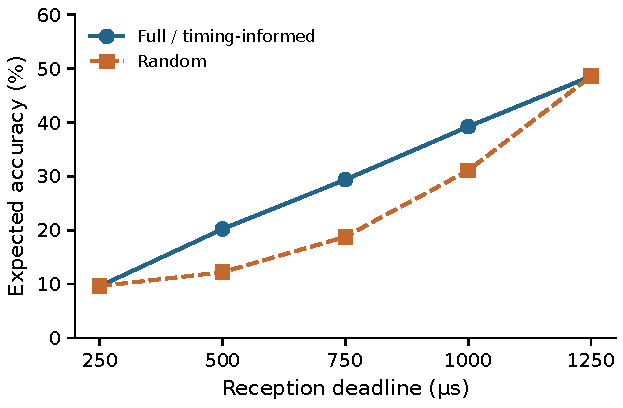
\includegraphics[width=\linewidth]{equal_cost_admission.pdf}
\caption{Equal offered cost can conceal different useful delivery. Values reproduce Table~\ref{tab:external_deadlines} for three frozen MNIST-sum policies. Timing-informed and random admission have matched offered bytes at each deadline; Full offers 17 bytes throughout. Lines show mean expected accuracy, not new evaluations; paired gain intervals are retained in the table.}\label{fig:admission}
\end{figure}

\subsection{Sender sensitivity versus selection advantage}\label{sec:selection}
To distinguish the relevance of sender identity from the quality of a particular choice, we compare feasible alternatives from the same state. At prespecified even timesteps on RR and DAC trajectories, we enumerate feasible one- or two-sender subsets with weights, full state and packet count fixed. Each branch resumes the factual scheduler afterward. Across 2,654 states, at least two alternatives differ in suffix return in 13.94--18.86\% of sampled states. That range establishes sensitivity; it does not show that the factual choice is better than alternatives.

For state $x$, feasible subsets $\mathcal A_{k(x)}$ and suffix return $V_x(A)$, the factual-minus-uniform contrast is
\begin{equation}
 \delta(x)=V_x(A_{\rm factual})-
 \frac{1}{|\mathcal A_{k(x)}|}\sum_{A\in\mathcal A_{k(x)}}V_x(A).
 \label{eq:subset_contrast}
\end{equation}
For sampled states $X_{s,e}$ in episode $e$ of seed $s$, the two averages are
\begin{align}
 \delta_s^{\rm state}&=
 \frac{\sum_e\sum_{x\in X_{s,e}}\delta(x)}{\sum_e|X_{s,e}|},\\
 \delta_s^{\rm episode}&=
 \frac{1}{E_s}\sum_e\frac{1}{|X_{s,e}|}\sum_{x\in X_{s,e}}\delta(x).
 \label{eq:subset_weighting}
\end{align}
Both final estimates weight seeds equally. State weighting emphasizes longer trajectories; episode weighting asks about a sampled decision in an equally weighted episode. Neither estimates replacing the scheduler at every future step, which would change the visited-state distribution.

All four episode-weighted intervals include zero (Table~\ref{tab:sender_weighting}). DAC-trained policies gain 0.13 points on Slow/5 ms and lose 0.25 on Medium/2 ms, with intervals $[-0.06,0.32]$ and $[-0.64,0.14]$. Two state-weighted intervals exclude zero. Thus sender identity matters in some states, but the tested factual priorities have no resolved episode-weighted advantage over uniform feasible substitutions.
\begin{table}[htbp]\centering\normalsize
\setlength{\tabcolsep}{4pt}
\caption{A sender can matter without the factual rule having a resolved advantage. Each row uses ten training seeds and ten evaluation resets per seed. Effect is the seed-mean percentage of sampled states with different feasible-subset returns. The last two columns estimate Eq.~\eqref{eq:subset_contrast} under the two weightings. Brackets are unadjusted 95\% Student-$t$ intervals across seeds; branches are paired alternatives.}\label{tab:sender_weighting}
{\footnotesize\setlength{\tabcolsep}{1.3pt}\begin{tabular}{llrlll}\toprule
Condition & Weights & States & Effect (\%) [CI] & Factual $-$ uniform, state & Factual $-$ uniform, episode\\\midrule
Slow/5 ms & RR & 646 & 18.86 [15.33, 22.40] & $-0.056$ [$-0.277$, $0.166$] & $-0.178$ [$-0.526$, $0.171$]\\
Slow/5 ms & DAC & 687 & 13.94 [9.45, 18.44] & $0.182$ [$0.008$, $0.356$] & $0.130$ [$-0.064$, $0.324$]\\
Medium/2 ms & RR & 661 & 16.97 [9.99, 23.94] & $0.235$ [$0.100$, $0.371$] & $0.195$ [$-0.027$, $0.418$]\\
Medium/2 ms & DAC & 660 & 18.16 [11.13, 25.19] & $-0.145$ [$-0.439$, $0.149$] & $-0.249$ [$-0.636$, $0.139$]\\
\bottomrule\end{tabular}}
\end{table}

Withholding a delivered update asks a different question: the attempt stays charged, the previous cache entry remains, and no substitute fills the slot. Some branches change return, but all four signed intervals include zero because positive and negative effects can cancel. Dependence on an update, sensitivity to its replacement and superiority of its selection are distinct. Supplementary Sections~S3 and S8 retain withholding effects, branch denominators, seed distributions and the diagnostic figures.

\subsection{Inherited history and receiver memory}\label{sec:history}
The buffered-reception designs discussed in Section~\ref{sec:related} motivate a history control. Switching access at reset changes the entire reception history. To isolate a later choice, we branch after a common RR prefix once every sender has a valid cache entry. The two branches inherit environment, recurrent, cache and scheduler state and remaining horizon. Prefix costs and episodes terminating before the branch remain in the episode averages, with zero suffix contrast for early terminations.

Across both weight sets, Slow/5 ms has zero DAC--RR return contrast in all 400 shared-prefix pairs despite changed action histories. At Medium/2 ms, return differs in 15 of 400 pairs. The RR-trained and DAC-trained episode means are $+0.350$ and $-0.350$, respectively, and both intervals include zero (Table~\ref{tab:history_by_cohort}). A cold episode-level contrast therefore need not persist after a common history.
\begin{table}[htbp]\centering\normalsize
\caption{Changing the same access rule at different points in a trajectory. All differences are DAC minus RR with the indicated frozen weights and fixed readiness. Each row has ten training seeds and 20 paired resets per seed. The prefix comparison includes episodes that terminate before full sender coverage; its intervals use the ten seed means. Cold-start values are means.}\label{tab:history_by_cohort}
{\footnotesize\setlength{\tabcolsep}{1.3pt}\begin{tabular}{llrrr}\toprule
Condition & Weights & Switch at reset & Switch after shared history [95\% CI] & Prefix survivors\\\midrule
Slow/5 ms & RR & $-0.850$ & $0.000$ [$0.000$, $0.000$] & 183/200\\
Slow/5 ms & DAC & $0.200$ & $0.000$ [$0.000$, $0.000$] & 190/200\\
Medium/2 ms & RR & $-1.700$ & $0.350$ [$-0.235$, $0.935$] & 199/200\\
Medium/2 ms & DAC & $-0.200$ & $-0.350$ [$-1.025$, $0.325$] & 200/200\\
\bottomrule\end{tabular}}
\end{table}

The zero Slow effect is not explained by universally exhausted reward opportunities. A privileged full-state reference achieves the predicted feasible suffix rewards: 296 endpoints allow 10 additional reward, 39 allow 20 and 65 allow none; Medium counts are 260, 139 and one. This measures remaining opportunity, not the performance of the frozen policies.

A separate ten-RR-checkpoint intervention clears cache payloads and validity timestamps at the common Slow endpoint, crossing retained/reset memory with RR/DAC continuation on 200 resets, including 17 early terminations. Removing memory changes actions in 154/200 RR and 155/200 DAC pairs. Every suffix return remains zero in all four branches. This demonstrates behavioral use of memory but cannot establish that cache mediation explains an earlier return contrast. The common prefix controls a whole trajectory; direct cache removal targets one component. Table~\ref{tab:memory_reset} reports the memory intervention; Supplementary Section~S8 retains the comparison of reset-time versus shared-prefix switches.
\begin{table}[htbp]\centering\normalsize
\caption{Direct memory removal at the common Slow/5 ms RR-prefix endpoint: ten RR checkpoints and 200 resets, including 17 early terminations. All four retained/reset $\times$ RR/DAC branches have zero suffix return in every episode. Action differences compare cleared with retained memory under the same subsequent access rule.}\label{tab:memory_reset}
\begin{tabular*}{\textwidth}{@{\extracolsep{\fill}}lrr@{}}\toprule
Later access & Changed histories & Changed returns\\\midrule
RR & 154/200 & 0/200\\
DAC & 155/200 & 0/200\\
\bottomrule\end{tabular*}
\end{table}

\subsection{Computation changes reception opportunities}\label{sec:timing}
At Medium/2.25 ms, a third 48-byte packet requires readiness within 310 microseconds after allowing 450 microseconds post-reception reserve, 50 microseconds propagation and 1.44 ms serialization. Mean RR/DAC gate times are 128.7/208.4 microseconds. Delivered counts are 2.175/1.999 under measured readiness but 2.000/2.000 under fixed 500-microsecond readiness. Common bandwidth and byte caps therefore do not ensure equal reception opportunity.

Three independent processes on the same pinned CPU, with ten seeds and three resets per cell, give episode-weighted RR means of 2.206, 2.005 and 2.002 at 2.25 ms, versus 2.000 for DAC in each repeat. On identical-input snapshots DAC adds 98--100 microseconds of episode-weighted gate work, with no delivered-count difference on those snapshots. Its extra computation is persistent; losing a packet depends on readiness tails, available credit and distance from the cutoff.

For three packets, the Medium-link preparation budget is $D_{\max}-1{,}940$ microseconds: 60, 310 and 560 at 2.00, 2.25 and 2.50 ms. In the original sweep, third-packet percentages for RR/DAC are 0/0, 17.5/0 and 49.3/49.8, averaging within episodes and then seeds. These measurements locate a discrete reception boundary rather than establishing a hardware-independent speed advantage. The diagnostic figure in Supplementary Section~S8 places the measured/fixed-readiness curves alongside the separate sender and history diagnostics.


\subsection{Available information and acting-policy use}\label{sec:receiver_decision}
The signaling/listening distinction motivates testing available information separately from the acting policy. We fit held-out linear probes~\citep{alain2016understanding} using ridge regression~\citep{hoerl1970ridge} on the actual receiver input. Earlier source-aware diagnostics reach 99.91--100\% decoding accuracy while actors achieve 64.17--78.44\% (Supplementary Section~S4). A probe identifies information; it does not execute a policy.

On normal RR access with ten Medium/2 ms checkpoints, an aggregate decoder fitted on ten episodes reaches 69.37\% on fresh resets, versus the unchanged actors' 56.58\%. The paired gap is 12.79 points [8.12, 17.47]. RR delivers the current source update on 40\% of steps. Independent source bits give expected accuracy one half otherwise, so even perfect decoding of timely updates has an expected ceiling of $0.40+0.60/2=0.70$. The use gap therefore persists without privileged source selection.

We fit only the follower head with 100 full-batch updates on 200 labeled bit observations (800 follower examples per seed/access rule). Source-head, encoder and scheduler parameters stay fixed. A shuffled-label control uses identical inputs and budget but permutes timestep labels jointly across followers. All 40 adapted/shuffled 4,930-parameter heads take 3.06 seconds to fit on the study CPU. Evaluation uses 20 fresh paired 20-step episodes per seed; the wrapper evaluates both heads for every treatment.

Normal accuracy rises from 56.58\% to 63.01\%, gaining 6.43 points [3.32, 9.54] over unchanged and 14.91 [10.04, 19.77] over shuffled heads. One seed loses 1.19 points. The shuffled actor achieves 48.10\%; probe decoding reaches 69.37\% (Table~\ref{tab:receiver_controls}; Fig.~\ref{fig:receiver_utilization}). These are ten-seed paired intervals after averaging episodes. Admission stays at 96 wire bytes and 64 delivered payload bytes per step, with matched sender identities/timestamps. Source-aware adaptation rises from 65.08\% to 87.74\%, but all its steps miss the action deadline; normal miss fractions are 1.63\% and 3.53\% for original and adapted wrappers.
\begin{table}[htbp]\centering\normalsize
\caption{Receiver adaptation with a matched shuffled-label control. Each access regime uses ten seeds, ten fit episodes and 20 fresh evaluation episodes per arm and seed. Accuracy and deadline misses are seed means in percent. The unchanged-input probe is fitted on the separate fit episodes and evaluated on inputs from the unchanged actor. All acting arms retain the same admission schedule within each regime.}\label{tab:receiver_controls}
{\footnotesize\setlength{\tabcolsep}{1.3pt}\begin{tabular}{llrr}\toprule
Access & Receiver & Accuracy (\%) & Action deadline misses (\%)\\\midrule
Normal RR & Unchanged & 56.58 & 1.63\\
Normal RR & True-label adaptation & 63.01 & 3.53\\
Normal RR & Shuffled-label adaptation & 48.10 & 2.05\\
Source-aware & Unchanged & 65.08 & 100.00\\
Source-aware & True-label adaptation & 87.74 & 100.00\\
Source-aware & Shuffled-label adaptation & 51.01 & 100.00\\\midrule
Normal RR & Probe of unchanged inputs & 69.37 & ---\\
Source-aware & Probe of unchanged inputs & 99.94 & ---\\
\bottomrule\end{tabular}}
\end{table}
\begin{figure}[htbp]\centering
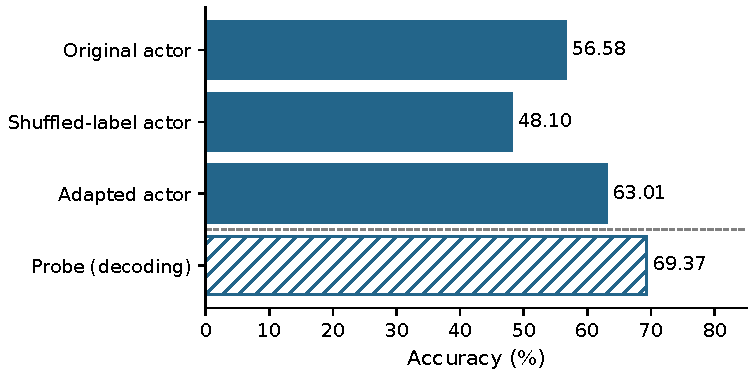
\includegraphics[width=\linewidth]{receiver_utilization.pdf}
\caption{Received information and behavioral utilization under normal RR access. Solid bars are actual closed-loop actor accuracy; the hatched bar is held-out decoding accuracy on unchanged-actor inputs, not an acting-policy score. Values reproduce Table~\ref{tab:receiver_controls}. This original fixed-readiness cohort executes candidates even if late; Fig.~\ref{fig:execution_boundary} separately reports hard fallback.}\label{fig:receiver_utilization}
\end{figure}

The update changes closed-loop behavior, not only predictions on frozen features. Source actions differ on 423/4,000 normal and 409/4,000 source-aware adapted steps despite unchanged source-head parameters. Follower actions enter subsequent recurrent inputs and can alter later messages. The result is the total effect of extra task-relevant supervision under a fixed access rule. Figure~\ref{fig:adaptation} retains the individual seed gains and paired intervals.
\begin{figure}[htbp]\centering
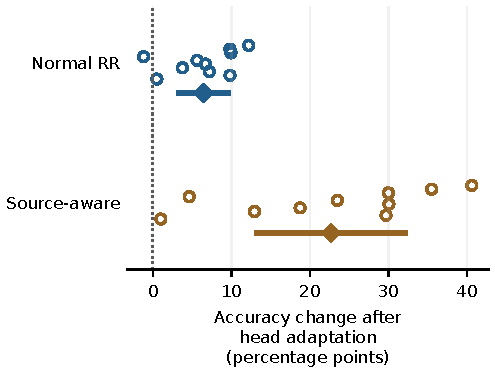
\includegraphics[width=\linewidth]{receiver_adaptation.pdf}
\caption{Change in acting accuracy on new broadcast episodes after fitting follower heads. Circles show each training seed's gain over the unchanged head, diamonds the ten-seed mean, and bars paired 95\% $t$ intervals. Normal RR supplies a current source update on 40\% of steps. Source-aware selection supplies it on all steps and incurs extra diagnostic CPU cost.}\label{fig:adaptation}
\end{figure}
 The original comparison executes late candidates; the next study tests actual rejection.

\subsection{Timing uncertainty and executed fallback}\label{sec:deployment_robustness}
Two frozen-policy follow-ups test assumptions behind the favorable admission and receiver contrasts, without new policy or head training. Supplementary Section~S7 gives their prerecording, complete settings and independent audit.

\paragraph{Readiness estimation with a decision cost}
For MNIST-sum, estimate $\hat r=r+b+\epsilon$, with $\epsilon\sim\mathcal N(0,\sigma^2)$ and sequential overhead $c$. Admission requires $\hat r+c+220\le D$ microseconds; actual arrival is $r+c+220$. We integrate noise and stochastic-policy probabilities exactly on the prior 1,024-pair cohort for each of three policies. Random admission matches expected offered bytes; the stronger reference has no extra prediction overhead.

At the predeclared primary setting $D=750$, $\sigma=100$, $b=0$, $c=100$, informed accuracy is 28.48\% versus 19.23\%, gaining 9.25 points [6.64, 11.85] at 8.276 offered B per example. At $\sigma=800$, $c=400$, the gain reverses to $-1.35$ [$-1.87$,$-0.82$]. All 450 settings are retained. Three-seed intervals condition on test pairs and the error model. Marginalizing random masks gives a zero-error/zero-overhead contrast of 9.88 rather than the original finite-mask 10.59 points. Full without decision cost still scores 29.37\% at the primary setting: robustness against random admission does not retain Full--informed identity.

\paragraph{Replacing late candidate actions}
Ten broadcast policies and saved heads run on 20 new paired resets per seed, with measured readiness and a 2 ms deadline. Late candidates are replaced by the previous executed joint action (initially zero) or the all-zero action. Executed actions feed the next recurrent input; cache and hidden state persist. Three serial CPU processes are averaged within seed before ten-seed inference, rather than treated as 30 seeds.

Previous-action fallback with no added cost gives 57.69\% original and 63.31\% adapted accuracy, a 5.63-point gain [1.80, 9.46]. Candidate miss rates are 0.100\% and 0.058\%; every late candidate is rejected. The adapted-minus-shuffled gain is 16.39 points [9.27, 23.50]. Both lower bounds are positive in each process, although two training seeds lose accuracy. This establishes a conditional gain with rare overruns, not robustness to frequent violations or faster adapted computation.

Adding 250 microseconds postprocessing retains a 5.45-point gain [1.99, 8.92]. At 500 microseconds, every candidate is late and either fallback gives 47.75\% for every head, eliminating the gain (Fig.~\ref{fig:execution_boundary}). Ordinary late execution would still show 5.58 points. Privileged source-aware selection likewise has 100\% late candidates and zero gain after rejection; its fixed readiness is kept separate from measured normal access. Readiness error and overhead are modeled, and fallback is assumed preinstalled at the actuator. Rejecting late candidates is not a continuous-time hardware guarantee.
\begin{figure}[htbp]\centering
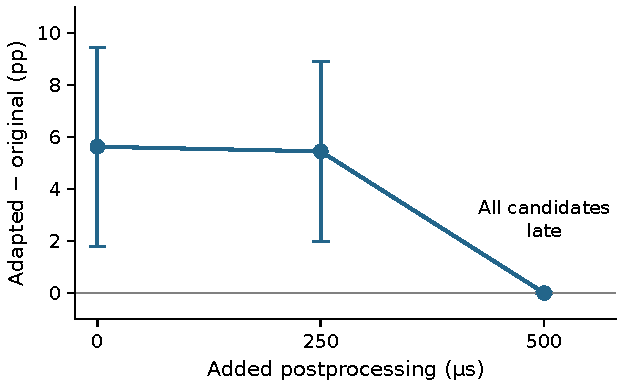
\includegraphics[width=\linewidth]{execution_boundary.pdf}
\caption{Receiver benefits depend on execution cost. Normal RR broadcast with measured readiness and previous-action fallback at a 2 ms deadline; ten seeds and three serial CPU processes. Points are paired adapted-minus-original accuracy gains, with 95\% seed-level $t$ intervals after averaging processes within seed. At 500 microseconds of added postprocessing, every candidate is late and every head achieves 47.75\%, giving exactly zero gain.}\label{fig:execution_boundary}
\end{figure}

\section{Discussion and conclusion}\label{sec:discussion}
Our analysis identifies limits of interpretation, rather than a common empirical failure of the cited methods. The literature supplies concrete targets: communication overhead, access selection, retained messages, waiting time and behavioral listening. Our experiments show which additional observations distinguish mechanisms behind those targets under the specified deadlines. Traffic reduction can remove only unusable offers; sender relevance can coexist with an unresolved selection advantage; and receiver information can improve supervised control only while actions remain executable.

The comparisons distinguish three design decisions. When reception histories are identical, traffic can be reduced by removing unusable offers without changing policy information. When received histories differ, selection claims require a specified counterfactual and averaging unit: sender sensitivity, episode-weighted advantage and dependence on a cached history are separate quantities. When received information is decodable but underused, an acting-head intervention can test a receiver change, provided its labels, feedback and computation are included in the claim.

The framework consequently connects a performance difference to the component that may warrant modification. It does not decompose return additively or identify every mechanism. The memory intervention illustrates this limit: changed actions with zero suffix reward demonstrate a behavioral effect but leave cache mediation unresolved. Similarly, positive supervised receiver gains do not establish improved communication alone, and a nominally matched link does not account for the computation needed to exploit it.

Scope remains restricted to Oracle-assisted five-agent Hallway, Oracle-free five-agent broadcast and the one-step MNIST-sum reconstruction. Hallway is solvable without communication and requires clonable full state for replay; enumerating sender alternatives costs $\binom Nk$ suffix rollouts per state. MNIST admission initially knows readiness without prediction cost; the follow-up models estimator error rather than implementing a predictor. Broadcast adaptation uses current-bit labels. CPU results cover one host. Transport is serial and simulated, with no retries, backlog or compute/transfer overlap and no physical score-collection traffic. Original late-execution results and hard-fallback results remain distinct.

Negative learning and transfer checks further bound the conclusions. XOR failed in all ten seeds. An early SMACv2 pilot~\citep{ellis2023smacv2} failed; a later three-seed Terran campaign passed at 300,000 steps, but independent-engine replay failed at the second seed after 320 evaluation episodes. A separate one-checkpoint smoke verified instrumentation over 20 episodes and 1,046 steps, including one 47-step Full--RR identity. It supplies no multi-seed paired learned-policy effects (Supplementary Section~S5).

Within these limits, offered traffic and return remain useful system summaries, but support different explanations only when delivery, sender history, CPU readiness and executed action are observed or controlled. The four-stage protocol supplies those comparisons and preserves unsuccessful tests alongside favorable ones. Establishing their prevalence and magnitude on learned standard sequential benchmarks, larger populations and physical channels remains future work.

\FloatBarrier
\section*{Statements and Declarations}

\subsection*{Funding}
No specific funding was received for this work.

\subsection*{Competing interests}
The authors declare no competing interests.

\subsection*{Author contributions}
\textbf{Yeong-woo Kung:} Conceptualization, Methodology, Software, Validation, Formal analysis, Investigation, Writing -- original draft. \textbf{Young-guk Ha:} Supervision, Project administration, Writing -- review \& editing.

\subsection*{Data availability}
The generated data, trained checkpoints and evaluation outputs are available in the \texttt{data/}, \texttt{checkpoints/} and \texttt{results/} directories of the repository linked below, with a file-level checksum manifest and reproduction instructions. A portable reviewer archive can also be generated from that repository. Raw MNIST images are obtained separately using the repository's checksum-verified download instructions; the StarCraft II runtime is not redistributed.

\subsection*{Code availability}
The code for this study is available at \url{https://github.com/yeongwookung07-eng/Evaluating-Deadline-Limited-Communication-in-Multi-Agent-Reinforcement-Learning}.
\setlength{\bibsep}{1pt plus1pt}
\bibliography{references}
\clearpage
\section*{Authors and affiliations}
\textbf{Yeong-woo Kung}\par
First author\par
E-mail: \href{mailto:yeongwoo@konkuk.ac.kr}{yeongwoo@konkuk.ac.kr}\par
\vspace{12pt}
\textbf{Young-guk Ha}\par
Second and corresponding author\par
E-mail: \href{mailto:ygha@konkuk.ac.kr}{ygha@konkuk.ac.kr}\par
\vspace{16pt}
\textbf{Affiliation of both authors}\par
Smart Computing Laboratory, Department of Computer Science \& Engineering, Konkuk University, 120 Neungdong-ro, Gwangjin-gu, Seoul 05029, Republic of Korea.

\end{document}
